\section{Building blocks. The programs ``inside'' GNS3}
\label{sec:gns3buildingblocks}

In an very simplified way, GNS3 is a conjunction of UI/client tools (the official GUI, the new web UI, or any custom program that ``speaks'' the documented public \acrshort{rest} API), a powerful distributed orchestrator (the \emph{controller} in the server), and a set of integrations (the so-called ``compute nodes'') with virtualization and hardware emulation tools from ``the outside,'' i.e. that do not belong to the GNS3 project, like KVM, Docker, or QEMU, to provide a way to describe a topology of interconnected computing and routing nodes---that is, a computer network---, including firewalls and NAT devices, control their behavior and launch administrative tools (like \texttt{telnet} sessions). % TODO cite documentation of the REST API. Make sure we elaborate on "computes". How is so-called written - is an hyphen used?

% What follows is a description of what are those elements and what they do work internally.
% How they integrate with GNS3 or vice-versa, and also how they interact with each other, is described in~\ref{sec:gns3architecture}.

\begin{figure}
  \centering
  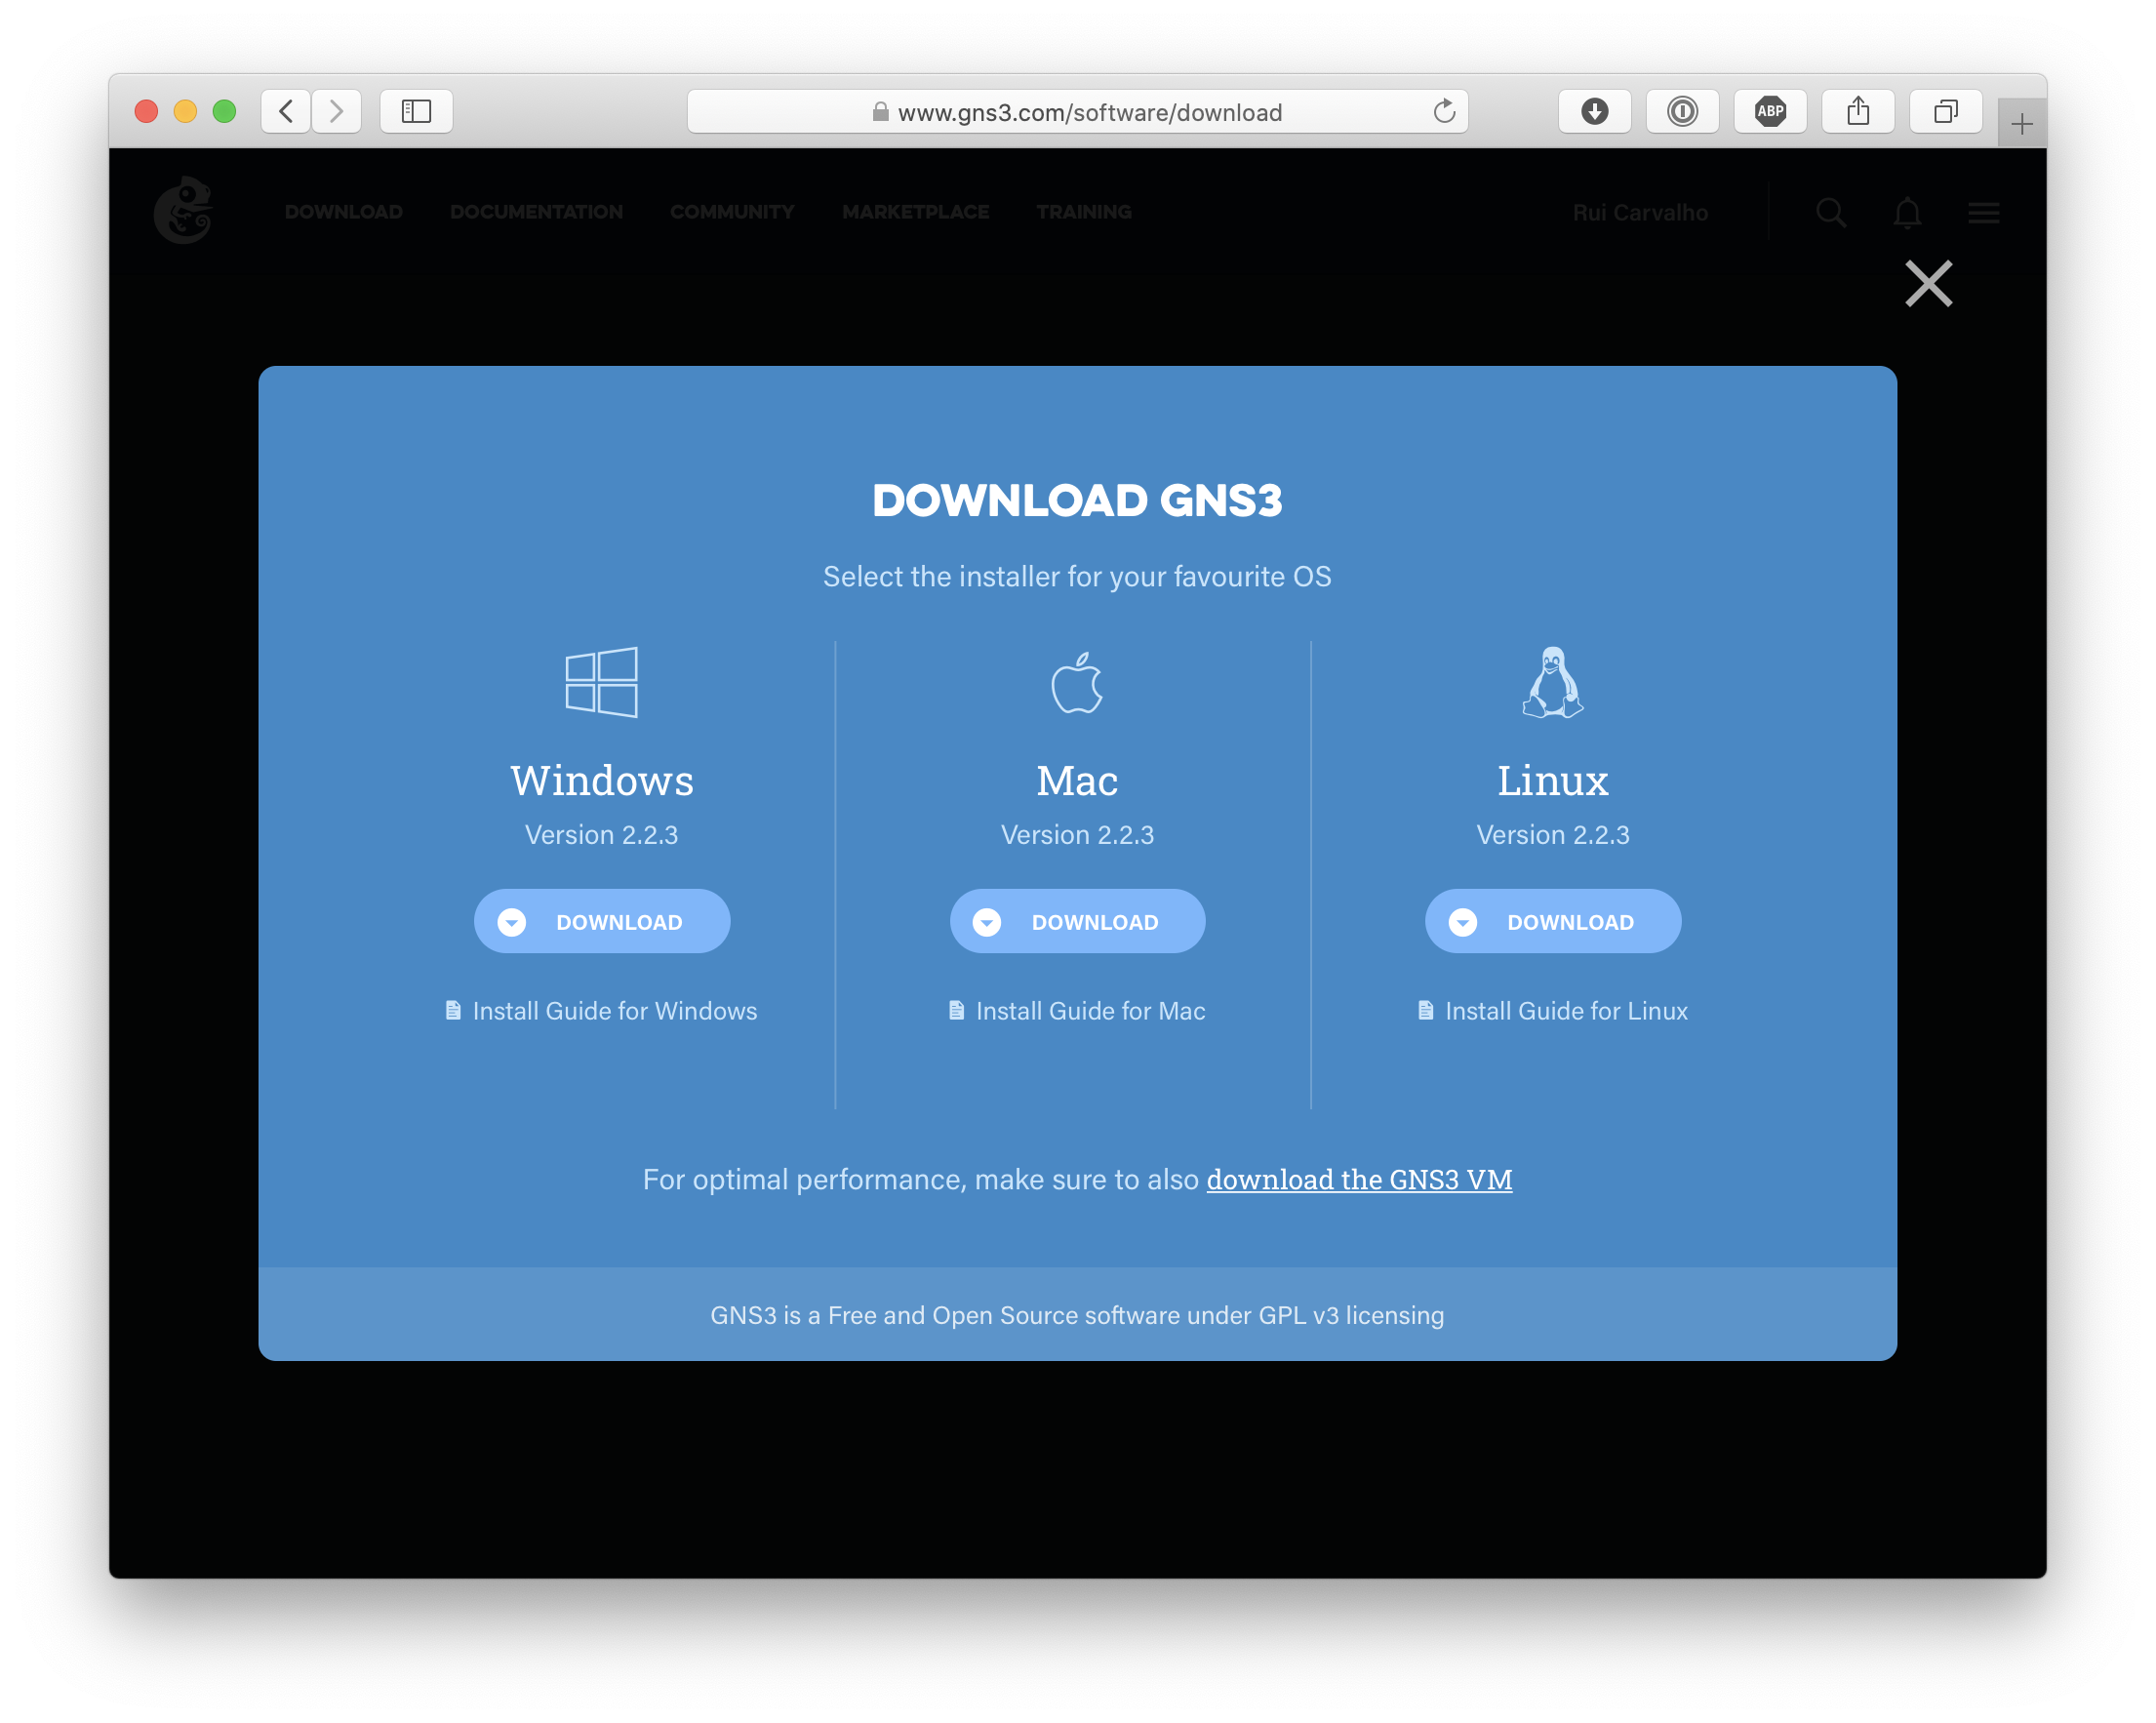
\includegraphics[width=0.8\textwidth]{download-gns3}
  \caption{The download screen on the official GNS3 website}
  \label{fig:download-gns3}
\end{figure}

When GNS3 is installed downloading one of its desktop distributions---available for Windows, macOS, and GNU/Linux, like the screen shot~\ref{fig:download-gns3} shows---, a user is installing multiple ``programs'' (or applications, whichever is the preferred denomination), implemented in disjunct codebases, and, given that they are \emph{free and open source} projects~\cite{gplv3}, hosted in GitHub, are easily accessible---and developers can enhance features and provide bugfixes.
Those are the essential building blocks of GNS3 and table~\ref{tab:gns3components} can serve a summary of what those pieces are.
It's worth noting that they are all under the GNS3 organization in GitHub\footnote{\url{https://github.com/gns3}}.

\begin{table}
  \centering
  \small
  \begin{tabulary}{0.95\textwidth}{lLL}
    \toprule
      \textbf{Part}       & \textbf{Role}                                                           & \textbf{Source code repository URL}\\
    \midrule
      GNS3 GUI            & A desktop application that runs on a graphical OS                       & \scriptsize\url{https://github.com/GNS3/gns3-gui}\\
      GNS3 server         & The main \emph{backend} implementation of GNS3. Its decision point      & \scriptsize\url{https://github.com/GNS3/gns3-server}\\
      Dynamips            & A MIPS emulator able to run legacy IOS images                           & \scriptsize\url{https://github.com/GNS3/dynamips}\\
      uBridge             & Application to bridge different user-land bridges                       & \scriptsize\url{https://github.com/GNS3/ubridge}\\
      VPCS                & A simulator for a real PC, with a few implemented commands              & \scriptsize\url{https://github.com/GNS3/vpcs}\\
    \bottomrule
  \end{tabulary}
  \caption{%
    Parts of GNS3, constituting separate and independent codebases
  }
  \label{tab:gns3components}
\end{table}


\subsection{GNS3 GUI}
\label{subsec:gns3gui}

Interaction between the end-user and GNS3 is usually---though, as will be clear, not necessarily---done in a graphical environment.
A GNS3 project, called a \emph{topology}, is constantly opened on one single window (per running instance of the application) and is graphically represented in the main section of the window.

Even though the GUI is not the authoritative source of truth for a topology (cf.~\ref{sec:gns3architecture}), it can be used as interface to all of GNS3's functionality: edit the topology itself (adding or removing nodes, changing links), performing actions on the nodes (like starting or stopping a host or router), or using helpers to launch consoles automatically connected via \texttt{telnet} or SSH.
In the section dedicated to the usage of GNS3~\ref{sec:gns3inaction}, it will be shown how this is done from a user's perspective.
Many GUI clients, on different hosts (e.g. laptops), can be editing the same topology at the same time. % TODO try to capture screenshots of this happening (use VMs)

\begin{figure}
  \centering
  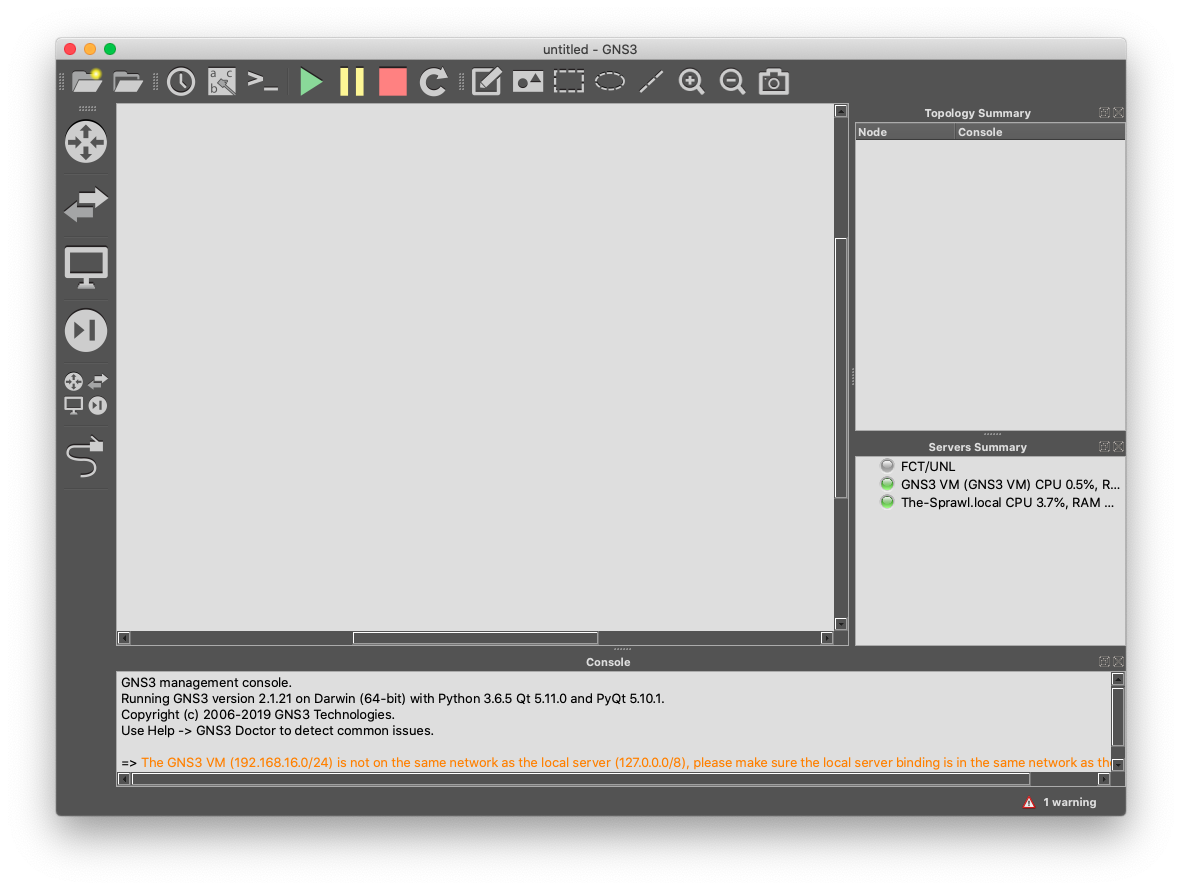
\includegraphics[width=0.8\textwidth]{gns3-empty-topology}
  \caption{An empty GNS3 topology shown in the GUI}
  \label{fig:gns3-empty-topology}
\end{figure}

\subsection{Dynamips}
\label{subsec:gns3dynamips}

The Dynamips emulator is a standalone program, written in C, that, usually, comes distributed together with the whole GNS3 package.
It is an emulator for a MIPS processor and was the original--single way to run the software of the Cisco nodes of the topologies created with GNS3.


\subsection{GNS3 server}
\label{subsec:gns3server}


\subsection{GNS3 VM}
\label{subsec:gns3vm}

% end of section gns3buildingblocks
